% manuscript.tex — Journal of Simulation submission (double-anonymous)
% Template: Taylor & Francis Interact layout + Reference Style P (tfp.bst)
% All quantitative claims are mechanically verified against results/*.csv
% by scripts/verify_consistency.py (commit c0ae64e); see Appendix A.
%
% NOTE TO AUTHORS (remove before submission):
%  - Real author block: uncomment and complete below for the version with
%    author details; the submitted PDF must be the anonymous one.
%  - Confirm the Funding / Generative AI declarations before submitting.

\documentclass[]{interact}

\usepackage{epstopdf}
\usepackage{amsmath}
\usepackage{amsthm}
\usepackage{graphicx}
\usepackage{booktabs}
\usepackage{url}
\usepackage{algorithm}
\usepackage{algpseudocode}

\newtheorem{lemma}{Lemma}
\newtheorem{proposition}{Proposition}
\newtheorem{corollary}{Corollary}

\usepackage[numbers,sort&compress,merge]{natbib}
\bibpunct[, ]{(}{)}{,}{n}{,}{,}
\renewcommand\bibfont{\fontsize{10}{12}\selectfont}
\renewcommand\citenumfont[1]{\textit{#1}}
\renewcommand\bibnumfmt[1]{(#1)}

\begin{document}

\articletype{Research Article}

\title{Protection level or behavioural dynamics? An effect-decomposition study of an information-saliency-driven hybrid simulation framework for dengue}

% ----- Real author block (for the with-authors version) -----
% \author{
% \name{[Author One]\textsuperscript{a}\thanks{CONTACT [Author One]. Email: [email]}}
% \affil{\textsuperscript{a}[Department, University, City, Country]}
% }

\author{
\name{[Author details removed for double-anonymous peer review]}
\affil{[Affiliation removed for double-anonymous peer review]}
}

\maketitle

\begin{abstract}
Behaviour-coupled epidemic models are usually evaluated by comparing simulations with and without an endogenous behavioural feedback, which confounds the contributions of protective-behaviour level and dynamics. We built a four-layer hybrid simulation framework for dengue---agent-based individuals, system-dynamics transmission, discrete-event hospital resources, and explicit mosquito dynamics, both channels modulated by population protection---and evaluated it with an effect-decomposition design: a constant-protection control arm, a mechanism control swapping the saliency module for a prevalence-tracking awareness module at matched protection, paired-seed ablation, calibration with transfer tests on Brazilian surveillance data, and a scale replication. The behavioural feedback flattened the epidemic (peak reduction 35.9\% at $N{=}1{,}000$; 24.8\% at $N{=}10{,}000$), but constant protection reproduced 95\% (85\% at scale) of it; the saliency-driven dynamics added a small, non-significant margin (3.2 points). At matched protection, the awareness control extracted a significant dynamic margin of 22.5 percentage points. Analytically, a two-channel invasion threshold ($R_0{=}3.16$) shows the information channel cannot block invasion, and a midpoint-invariant protection-band bound explains why its dynamics are structurally narrow while the awareness module's are not. Calibration reached $R^2=0.941$ and transferred to large epidemic seasons only. The decomposition design is offered as a diagnostic standard for such models.
\end{abstract}

\begin{keywords}
hybrid simulation; agent-based modelling; dengue; behavioural epidemiology; model validation; effect decomposition
\end{keywords}

\section{Introduction}

Dengue is the fastest-spreading mosquito-borne viral disease in the world, with roughly three billion people at risk of infection \cite{kraemer2019past}. In the absence of widely deployed vaccines or specific therapeutics, control relies on vector management and on the protective behaviour of exposed populations---mosquito-avoidance measures, source reduction, and care-seeking behaviour \cite{esteva1998analysis}. Because such behaviour responds to the information environment---media coverage, public communication, and observed illness in one's surroundings---there is a long research tradition of coupling information spread to epidemic dynamics \cite{funk2009spread,funk2010modelling,perra2012activity}. A recurring result of this literature is that adaptive human behaviour can alter epidemic trajectories substantially, to the point that ignoring it misestimates both peaks and final sizes \cite{fenichel2011adaptive}.

How such behaviour-coupled models are \emph{evaluated}, however, has received far less attention than how they are built. The standard evaluation compares a simulation in which the behavioural feedback is enabled against one in which it is disabled, with protection effectively fixed at zero. Any resulting difference is then attributed to ``the behavioural mechanism''. This comparison cannot distinguish between two very different claims: that the population exhibits some average level of protection, and that the \emph{time-varying, information-driven} dynamics of that level carry epidemiological value beyond the level itself. The distinction matters practically. If the level carries the effect, interventions should be judged by whether they raise and sustain protection; if the dynamics carry it, the timing and shape of information interventions become the object of design. Fenichel et al.\ \cite{fenichel2011adaptive} made the theoretical case that adaptive versus static behaviour leads to different epidemic predictions, which suggests the distinction is substantive---yet applied simulation studies rarely report the controls needed to see which side of it their own model falls on.

A second strand of literature motivates the modelling vehicle rather than the evaluation. Single-paradigm models face a structural trade-off: system-dynamics (SD) models are tractable but assume homogeneous mixing; agent-based models (ABMs) capture heterogeneity and behaviour but are costly and hard to calibrate. Hybrid simulation combines paradigms within one model. Reviews of hybrid simulation in health care report that DES--SD is the most common combination, that the full ABM--DES--SD combination remains early-stage, and that existing applications concentrate on hospital operations and patient flow rather than on coupling to disease transmission and information-driven behaviour \cite{kar2025hybrid}. Hybrids that mix only two paradigms have been catalogued and classified \cite{borshchev2004system,morgan2017toolkit}, and ABMs of epidemic spread in realistic contact structures are well established \cite{eubank2004modelling,ferguson2020impact,prem2020effect,chinazzi2020effect}. What is missing is a framework that couples information-driven behaviour, resource constraints, and vector dynamics in one model, evaluated with a design that can attribute effects to components.

This paper presents such a framework and, more importantly, the evaluation design we used to interrogate it. The framework couples four layers: an ABM of individuals whose risk perception---driven by an information-saliency signal, social influence, and personal experience---produces protective behaviour; an SD transmission core; a discrete-event (DES) layer for hospital beds and ICU capacity; and an explicit mosquito-dynamics layer, since dengue is vector-borne. Both transmission channels are modulated by the population mean protection level through a protection-efficiency parameter. The evaluation is organised around six questions: (RQ1) does the information--behaviour feedback flatten the epidemic; (RQ2) how much of that effect is carried by the protection \emph{level} versus its \emph{dynamics}, and does the answer survive a ten-fold increase in population; (RQ3) is the small dynamic margin a property of behavioural dynamics in general or of our saliency parameterisation in particular; (RQ4) how much media amplification would be needed to reach a pre-specified effect target; (RQ5) does the model calibrate to real surveillance data, and does the calibration transfer across seasons; and (RQ6) which components carry the system behaviour.

Answering these questions required three design elements that, while individually established in adjacent literatures---static-versus-adaptive comparisons appear in the optimal-control tradition \cite{fenichel2011adaptive}, and awareness modules in the awareness--epidemic tradition \cite{funk2009spread}---are rarely combined inside a behaviour-coupled epidemic simulation: a constant-protection control arm calibrated to the endogenous model's own mean protection (RQ2); a mechanism control that swaps the saliency-driven behavioural module for a prevalence-tracking awareness-diffusion module at matched mean protection (RQ3); and a deterministic surrogate of the agent-based model's expectation dynamics that makes grid-search calibration on real data tractable, with frozen-parameter out-of-season transfer tests (RQ5). All experiments run under a seeded regeneration protocol, and every quantitative claim in this paper is mechanically checked against archived output files by a consistency script.

The paper's findings are deliberately reported with their boundaries. The feedback does flatten the epidemic, but a constant protection level reproduces 95\% of the effect at $N{=}1{,}000$ and 85\% at $N{=}10{,}000$; the saliency-driven dynamics contribute a small, non-significant margin at the smaller scale that becomes significant but still minor at the larger one. The mechanism control shows that this is not a general truth about behavioural dynamics: at matched mean protection, a prevalence-tracking awareness module extracts a large, significant dynamic margin, locating the limitation in the saturating shape of our response function. Calibration on Brazilian 2019 weekly data reaches $R^2=0.941$ and transfers to large epidemic seasons but not to small years. We offer the decomposition design itself, together with the open protocol and consistency tooling, as the paper's principal methodological contribution.

\section{Related work}

\subsection{Epidemic simulation paradigms and hybrids}

Compartmental models remain the analytic backbone of epidemic modelling, but their homogeneous-mixing assumption limits behavioural realism. Agent-based models recover heterogeneity and behavioural decision-making; landmark applications include city-scale network simulations of smallpox \cite{eubank2004modelling} and the COVID-19 non-pharmaceutical-intervention studies \cite{ferguson2020impact,prem2020effect,chinazzi2020effect}, at the cost of computational expense and calibration difficulty. SD models occupy the opposite corner: tractable and policy-oriented \cite{sterman2000business}, with a mature validation methodology \cite{barlas1996formal}, but equally homogeneous.

Hybrid simulation mixes paradigms within one model, and the community has developed both the motivation and the design vocabulary for doing so. Borshchev and Filippov \cite{borshchev2004system} systematised why modellers move between SD, DES, and ABM within a single study---different abstraction levels answer different questions---and demonstrated practical coupling techniques. Morgan et al.\ \cite{morgan2017toolkit} turned mixed DES--SD practice into a toolkit of named designs with explicit assessment of opportunities and risks, providing the methodological vocabulary this paper borrows when it describes its layers and their coupling direction. In health care specifically, the systematic review of Kar et al.\ \cite{kar2025hybrid} found DES--SD to be the dominant combination, the full ABM--DES--SD combination rare, and existing applications concentrated on hospital operations and patient flow rather than on coupling to disease transmission and information-driven behaviour. Applications coupling a hybrid model to disease transmission, vector dynamics, and information-driven behaviour have, to our knowledge, not been reported; dengue adds the specific requirement of an explicit vector layer \cite{esteva1998analysis}, which is absent from the hybrid-simulation portfolio the review covers.

\subsection{Behaviour, information, and epidemics}

That information changes epidemics is well established. Funk et al.\ \cite{funk2009spread} coupled awareness spread to transmission and showed that awareness can reduce outbreak sizes; their review \cite{funk2010modelling} consolidated the modelling approaches, and the subsequent systematic review of Verelst et al.\ \cite{verelst2016behavioural} catalogued the 2010--2015 generation of behavioural-change models, noting that most couple behaviour to transmission through a reduced-susceptibility or reduced-contact channel driven by prevalence---the same structural slot our saliency channel occupies. Bedson et al.\ \cite{bedson2021review} set an agenda for integrated disease models that include social and behavioural factors and observed that such integration remains the exception in practice, particularly for vector-borne disease. Centola \cite{centola2010spread} and Bakshy et al.\ \cite{bakshy2012role} established the empirical mechanics of behaviour and information diffusion in networks, and Perra et al.\ \cite{perra2012activity} formalised adaptive behaviour--transmission coupling on time-varying networks, where behavioural adaptation alters epidemic thresholds and final sizes. On the psychological side, risk perception is a reliable but moderate predictor of protective behaviour \cite{rosenstock1974historical,rogers1975protection,ajzen1991theory,brewer2007meta,ferrer2015risk}---an effect size our behaviour model deliberately reflects by producing moderate protection levels rather than on-off adoption. Fenichel et al.\ \cite{fenichel2011adaptive} demonstrated theoretically that adaptive behaviour changes epidemic outcomes relative to static baselines---the closest methodological antecedent of our study, though without a simulation framework or an experimental decomposition; our mechanism control operationalises exactly the contrast they analyse.

\subsection{Positioning}

Against this background the paper positions itself on the evaluation side. First, we embed information-driven behaviour, hospital resources, and vector dynamics in one four-layer hybrid model (Section 3), extending the healthcare hybrid-simulation portfolio towards transmission coupling \cite{kar2025hybrid}. Second, and principally, we evaluate it with a decomposition design that separates protection level from protection dynamics, add a mechanism control drawn from the awareness literature, and report where our own mechanism fails. The design is generic: any behaviour-coupled epidemic model can be interrogated the same way.

\section{Model and methods}

\subsection{Framework overview}

The framework couples four layers (Figure~\ref{fig:framework}). The \emph{ABM layer} holds $N$ individual agents with discrete states $S$ (susceptible), $E$ (exposed), $I$ (infectious), and $R$ (recovered), a risk-perception value, and a protection level; state transitions are stochastic. The \emph{SD layer} provides the macroscopic information environment: an information-saliency signal computed from prevalence, media amplification, and decay, plus population-level risk perception with behavioural inertia. The \emph{DES layer} models hospital beds, ICU beds, testing capacity, and their queues; patients denied immediate admission are counted once as \emph{deferred admissions}, a resource-pressure metric. The \emph{mosquito layer} implements human--mosquito--human transmission with an explicit extrinsic incubation period.

Coupling is bidirectional. The ABM aggregates state counts and the population mean protection $P_{\mathrm{avg}}(t)$ upward; the SD layer feeds saliency into each agent's risk perception; the infection hazard of every susceptible agent depends on both transmission channels, each modulated by protection; the DES layer receives admission requests and returns admission outcomes. All experiments use population $N{=}1{,}000$, 200 simulated days, ten initial infections, and mosquito population $5N$ (a 5:1 mosquito-to-human ratio, preserved under scaling).

\begin{figure}[htb]
\centering
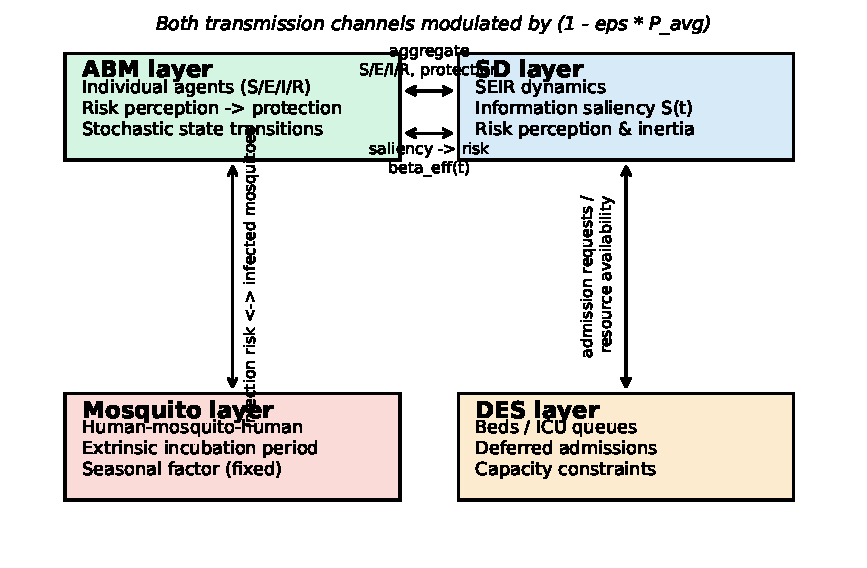
\includegraphics[width=0.95\linewidth]{figures/fig1_framework.pdf}
\caption{Four-layer hybrid simulation framework. Both the human-to-human and the mosquito-mediated transmission channels are modulated by the population mean protection $P_{\mathrm{avg}}$ through the protection-efficiency parameter $\varepsilon$.}
\label{fig:framework}
\end{figure}

\subsection{Information saliency, risk perception, and protection}

The information-saliency signal is a deliberately parsimonious two-parameter proxy for how salient the epidemic is in public perception:
\begin{equation}
S(t) = \min\!\left(1,\; \frac{I(t)}{N}\,\alpha\, e^{-\lambda t/100}\right),
\label{eq:saliency}
\end{equation}
where $\alpha$ scales media amplification and $\lambda$ governs decay. We note two caveats by design: the decay term is indexed by simulation calendar time rather than by information age, which is defensible only within a single epidemic wave (the decay factor stays in $[0.82,1]$ over 200 days), and neither $\alpha$ nor $\lambda$ is calibrated to media data; the contribution is a computable formalisation, not a measurement instrument.

Individual risk perception combines three sources---saliency, social influence (population prevalence), and personal experience (own or contacts' exposure)---with weights $w_{\mathrm{info}}{=}0.6$, $w_{\mathrm{soc}}{=}0.3$, $w_{\mathrm{pers}}{=}0.1$, updated with behavioural inertia $\eta{=}0.3$:
\begin{equation}
R(t) = (1-\eta)\,\big(w_{\mathrm{info}} S(t) + w_{\mathrm{soc}} \tfrac{I(t)}{N} + w_{\mathrm{pers}} E_{\mathrm{pers}}(t)\big) + \eta\, R(t{-}1),
\end{equation}
where $E_{\mathrm{pers}}$ indicates current or recent personal exposure. Protection follows a sigmoid response,
\begin{equation}
P(t) = \frac{1}{1+e^{-\kappa (R(t)-0.5)}}, \qquad \kappa = 1.5.
\label{eq:sigmoid}
\end{equation}
One property of Equation~(\ref{eq:sigmoid}) is central to everything that follows: its midpoint is fixed at $R{=}0.5$, so at near-zero risk it already yields $P\approx 0.32$. The population protection level therefore sits on the saturated shoulder of the curve, and the \emph{range} through which the information channel can move it is narrow. Section 4 quantifies the epidemiological consequences of this design choice.

\subsection{Two-channel transmission with protection modulation}

The human-to-human channel uses an effective transmission rate
\begin{equation}
\beta_{\mathrm{eff}}(t) = \beta_{\mathrm{base}}\,\big(1 - \varepsilon\, P_{\mathrm{avg}}(t)\big),
\label{eq:beta}
\end{equation}
with $\beta_{\mathrm{base}}{=}0.3$ and a protection-efficiency parameter $\varepsilon{=}0.85$: even universal protection leaves 15\% residual transmission, reflecting imperfect compliance (uneven repellent use, inconsistent net use, incomplete source reduction). This is a modelling assumption, not a measured quantity. Because personal protection against dengue is essentially mosquito avoidance, the mosquito-mediated channel is modulated by the same factor. Mosquito dynamics follow a difference system with biting rate $b{=}0.3$, human-to-mosquito and mosquito-to-human transmission probabilities $p_{hm}{=}0.5$ and $p_{mh}{=}0.4$, extrinsic incubation period 10 days, and mosquito lifespan 14 days; the seasonal factor is fixed at 1. The daily infection hazard of a susceptible agent is
\begin{equation}
h(t) = \min\!\Big(1,\; \beta_{\mathrm{eff}}(t)\frac{I(t)}{N} + \underbrace{b\,p_{mh}\frac{M_i(t)}{M}}_{\text{mosquito risk}}\big(1-\varepsilon P_{\mathrm{avg}}(t)\big)\Big).
\label{eq:hazard}
\end{equation}
We retain the human-to-human term as a deliberate simplification standing in for unmodelled transmission pathways; dengue transmission is primarily vector-borne, and the term's independent contribution is listed among the limitations.

\subsection{Hospital resources and accounting}

The DES layer manages ordinary beds (200), ICU beds (50), and testing capacity (100/day) with 7-day and 14-day stays. Admission requests arrive with daily probability 0.15 per infectious agent (20\% severe); patients who cannot be admitted immediately queue and are admitted when resources free up, and counted exactly once as \emph{deferred admissions}; agents who recover while queued leave the queue. In the present design admission does not isolate infectious agents, so resource constraints do not feed back into transmission; Section 4.6 quantifies this boundary explicitly, and coupling admission to transmissibility is future work. Algorithm~\ref{alg:daily} summarises the daily cycle.

\begin{algorithm}[htb]
\caption{Daily simulation step of the hybrid model}
\label{alg:daily}
\begin{algorithmic}[1]
\State aggregate agent states $(S,E,I,R)$; compute $S(t)$ by Eq.~(\ref{eq:saliency})
\ForAll{agents} \Comment{behaviour layer}
  \State update $R_i \leftarrow (1-\eta)\,R_{\mathrm{target}} + \eta\,R_i$; $P_i \leftarrow \sigma(\kappa(R_i - \mu))$
\EndFor
\State $\bar{P} \leftarrow \mathrm{mean}_i\, P_i$ \Comment{or fixed to $P^{*}$ in the constant-protection arm}
\State update mosquitoes: $E_m, I_m$ by the difference system; $\mathrm{risk}_m \leftarrow b\,p_{mh}\,(I_m/M)$
\State $\beta_{\mathrm{eff}} \leftarrow \beta(1-\varepsilon \bar{P})$; hazard $h \leftarrow \min(1, \beta_{\mathrm{eff}} I/N + \mathrm{risk}_m (1-\varepsilon\bar{P}))$
\ForAll{susceptible agents} \Comment{transmission layer}
  \State infect with probability $h$ (state $S \to E$)
\EndFor
\ForAll{exposed agents} $E \to I$ with probability $\sigma$;\quad \textbf{for all} infectious agents: $I \to R$ with probability $\gamma$
\EndFor
\ForAll{infectious agents} \Comment{DES layer}
  \State request test w.p.\ $d$; request admission w.p.\ $h_{\mathrm{adm}}$ (20\% ICU); queue and count deferred if full
\EndFor
\State process discharge events and admission queues; record metrics
\end{algorithmic}
\end{algorithm}

\subsection{Study design}

All experiments share a seeded regeneration protocol: every run draws an independent seed $s = 1000\,b + i$ for base seed $b$ and replicate index $i$; result files carry canonical names; a machine-readable run manifest records the code commit, seeds, and dependency versions for every rerun; and a consistency script re-derives every quantitative claim in this manuscript from the archived output files, blocking commits on mismatch (Appendix~A). Six experiments address the research questions; Table~\ref{tab:designs} summarises them.

\begin{table}[htb]
\centering
\small
\begin{tabular}{p{3.4cm}p{5.2cm}p{4.6cm}}
\hline
\textbf{Design} & \textbf{Arms / conditions} & \textbf{Question} \\
\hline
Switch comparison & Behavioural feedback on vs.\ off (protection $\equiv 0$); 20 replicates/arm & RQ1: does the feedback flatten the epidemic? \\
Decomposition & Full model vs.\ constant protection $P^{*}$ vs.\ zero protection; 20 replicates/arm; $P^{*}$ = the full model's time-averaged protection & RQ2: level or dynamics? \\
Mechanism control & Saliency--sigmoid module vs.\ awareness-diffusion module (matched mean protection $\approx 0.336$); $2\times3$ arms $\times$ 10 replicates & RQ3: whose dynamics matter? \\
Media-amplification sensitivity & $\alpha \in \{0.5,\dots,5\}$, 10 replicates/group; threshold search $\alpha \in [0.5,10]$ & RQ4: what amplification reaches a 20\% peak reduction? \\
Calibration \& transfer & Grid search on a deterministic surrogate; Brazil 2019 weekly data; frozen-parameter out-of-season tests 2016--2023 & RQ5: real-data fit and transfer? \\
Scale replication & Decomposition design at $N{=}10{,}000$; 20 replicates/arm & RQ2: scale robustness \\
Ablation & 6 conditions $\times$ 10 paired-seed replicates (beds 50, ICU 10) & RQ6: component attribution \\
Robustness & Awareness-parameter grid ($3\times3$) and response-shape sweep ($5\times2$); matched-protection comparisons & RQ3: robustness of the diagnosis \\
\hline
\end{tabular}
\caption{Experimental designs. Every condition within a design shares its seed set.}
\label{tab:designs}
\end{table}

Three elements deserve specification. First, the \emph{constant-protection arm} fixes the population mean protection at $P^{*}$, the time-averaged protection of the full model under identical seeds---an internally consistent target that introduces no free parameter---while agents' behaviour no longer updates. The dynamic margin of the information channel is the difference between the full model and this arm. Second, the \emph{mechanism control} replaces the saliency--sigmoid module with an awareness-diffusion module of the kind used in the awareness--epidemic literature (a representative implementation, not a reproduction of any specific published model): an awareness fraction $A(t)$ updates by contact contagion, prevalence-driven onset, and forgetting, $A(t{+}1)=\mathrm{clip}\big(A + p_A A\,S/N + q\,I/N - d_A A\big)$ with $p_A{=}0.25$, $q{=}0.8$, $d_A{=}0.1$, and protection $P(t)=mA(t)$ with the same $\varepsilon$-modulation. The multiplier $m$ is calibrated by bisection so that the dynamic arm's time-averaged protection matches the target within 0.004 ($m^{*}{=}0.497$), making the comparison fair at matched mean protection. Third, \emph{calibration} runs on a deterministic surrogate whose expectation dynamics are isomorphic to the agent model (the same transitions, mosquito difference equations, information--behaviour equations, and per-step Bernoulli hazard), because gradient-based optimisation on a stochastic objective is unsound. The surrogate is grid-searched over $(\beta,\sigma,\gamma,\alpha,I_0)$ against Brazil 2019 weekly reported cases (OpenDengue national extract, ``Total'' case definition, 52 weeks; population $2.11\times 10^{8}$, mosquito ratio preserved), with the reporting fraction $\rho$ solved per grid point in closed form by least squares. The fitted parameters are then verified in the agent model, and frozen-parameter transfer is tested on the 2016--2023 seasons (2020 missing from the extract), strictly with $I_0$ frozen and loosely with per-season $I_0$ reselected from the calibration grid.

\subsection{Theoretical analysis}

Three analytical results explain the empirical findings that follow; proofs are in Appendix~B and the invasion threshold is validated numerically against the agent model (Table~\ref{tab:theory}).

\begin{lemma}[Risk envelope]\label{lem:envelope}
With nonnegative weights, the population mean risk satisfies $0 \le \bar{R}(t) \le \bar{R}_{\max}$, where $\bar{R}_{\max} = \max_t \big[(w_{\mathrm{info}}\alpha + w_{\mathrm{soc}})\,\tfrac{I(t)}{N} + w_{\mathrm{pers}}\tfrac{E(t)+I(t)}{N}\big]$.
\end{lemma}

\begin{proposition}[Two-channel invasion threshold]\label{prop:threshold}
At the disease-free state with constant mean protection $\bar{P}$, the expected system has reproduction number
\begin{equation}
R_{\mathrm{eff}}(\bar{P}) = (1-\varepsilon \bar{P}) \cdot \frac{K_h + \sqrt{K_h^2 + 4\,K_{hv} K_{vh}}}{2},
\label{eq:reff}
\end{equation}
with $K_h = \beta_{\mathrm{base}}/\gamma$ (direct channel), $K_{hv} = b\,p_{hm}\,\tfrac{N}{M}\big/\gamma$ (human-to-mosquito per generation) and $K_{vh} = b\,p_{mh}\,L$ (mosquito-to-human per generation). With the paper's parameters, $R_0 = 3.16$ ($K_h{=}3.00$, $K_{hv}{=}0.300$, $K_{vh}{=}1.68$) versus $3.00$ for the human channel alone, and the early growth factor implied by the linearised system ($\lambda_{\max} = 1.104$ per day) agrees with the simulated early growth of the zero-protection agent model ($1.088 \pm 0.008$ over 20 replicates; 1.5\% relative deviation).
\end{proposition}

\begin{corollary}[Invasion-blocking protection]\label{cor:block}
$R_{\mathrm{eff}}(\bar{P}) \le 1$ requires $\bar{P} \ge \bar{P}^{\dagger} = (1-1/R_0)/\varepsilon = 0.804$ --- far above the protection band the information channel can reach (Lemma~\ref{lem:envelope}, Proposition~\ref{prop:band}). Endogenous information-driven protection therefore cannot prevent invasion in this parameterisation, whatever its dynamics; it can only flatten the wave.
\end{corollary}

\begin{proposition}[Protection-band bound and midpoint invariance]\label{prop:band}
For any trajectory, the population protection lies in $[\sigma(-\kappa\mu),\; \sigma(\kappa(\bar{R}_{\max}-\mu))]$, and its width is at most $\tanh(\kappa \bar{R}_{\max}/4)$, the supremum of $\sigma(x+\Delta)-\sigma(x)$ over $x$ for a logit range $\Delta = \kappa\bar{R}_{\max}$. The logit width $\kappa\bar{R}_{\max}$ is \emph{independent of the midpoint} $\mu$: moving $\mu$ translates the band without widening it.
\end{proposition}

Three consequences map directly onto the experiments. First, with $\kappa{=}1.5$ and the observed prevalence envelope, the bound is $0.094$ while the measured protection band is $0.049$ wide ($0.321$--$0.370$): the saliency channel cannot vary protection by more than a few percentage points in a single wave. Second, the $\mu$-invariance explains why the response-shape sweep (Section 4.3) leaves the dynamic margin essentially unchanged---an analytic property, not a coincidence of the default midpoint. Third, the awareness module escapes Proposition~\ref{prop:band} because its contact-contagion dynamics are not bounded by the risk envelope: its protection amplitude (0.49) exceeds the saliency bound five-fold, which is why it produces a significant dynamic margin at matched mean protection. Finally, since the reachable band tops out at $0.41$--$0.46 \ll \bar{P}^{\dagger}$, Corollary~\ref{cor:block} predicts that total infections are structurally insensitive to information-driven protection---precisely the attack-rate saturation observed at scale (Section 4.2).

\begin{table}[htb]
\centering
\small
\begin{tabular}{lc}
\hline
\textbf{Quantity} & \textbf{Value} \\
\hline
$K_h = \beta/\gamma$ (direct channel) & 3.00 \\
$K_{hv} = b\,p_{hm}(N/M)/\gamma$ & 0.300 \\
$K_{vh} = b\,p_{mh}\,L$ & 1.68 \\
$R_0$, two channels (Eq.~\ref{eq:reff}, $\bar{P}{=}0$) & 3.16 \\
$R_0$, human channel only & 3.00 \\
$\lambda_{\max}$, linearised daily system & 1.104 /day \\
Simulated early growth factor (20 replicates) & $1.088 \pm 0.008$ \\
Invasion-blocking protection $\bar{P}^{\dagger}$ & 0.804 \\
Protection-band bound $\tanh(\kappa \bar{R}_{\max}/4)$ & 0.094 \\
Measured protection band (full model) & 0.049 (0.321--0.370) \\
Awareness-module protection amplitude & 0.49 (0.004--0.497) \\
\hline
\end{tabular}
\caption{Theoretical quantities and their numerical validation (Propositions~\ref{prop:threshold} and \ref{prop:band}; validation experiment in the run manifest).}
\label{tab:theory}
\end{table}

\section{Results}

\subsection{The switch effect (RQ1)}

Enabling the information--behaviour feedback substantially flattens the epidemic (Figure~\ref{fig:switch}, Table~\ref{tab:switch}). Peaks fall from 222.35 to 142.55 infectious individuals at $N{=}1{,}000$ (35.9\%, Welch $t{=}-19.49$, $p{=}8.5\times10^{-21}$) and occur 18.5 days later; total infections fall by 7.1\%. Effect sizes against the zero-protection control are large (Cohen's $d{=}-6.16$, 95\% CI $[-8.25,-5.15]$), but this is an artefact of what the control is: zero protection contrasts \emph{any} endogenous protection with none, and the resulting $d$ must not be read as the effect of information saliency. Section 4.2 performs that separation.

\begin{figure}[htb]
\centering
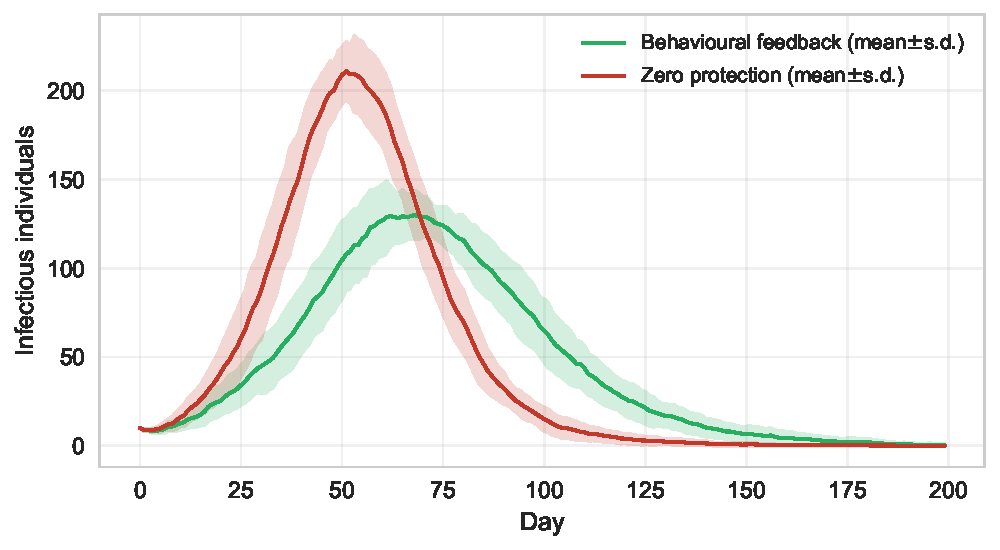
\includegraphics[width=0.85\linewidth]{figures/fig2_switch.pdf}
\caption{Switch comparison at $N{=}1{,}000$ ($n{=}20$ per arm): daily infectious counts, mean $\pm$ s.d.}
\label{fig:switch}
\end{figure}

\begin{table}[htb]
\centering
\small
\begin{tabular}{lcccc}
\hline
 & \textbf{Feedback} & \textbf{Zero protection} & \textbf{Reduction} & \textbf{Welch $t$ / $p$} \\
\hline
Peak infectious & $142.55 \pm 11.44$ & $222.35 \pm 14.30$ & $35.89\%$ & $-19.49$ / $8.5{\times}10^{-21}$ \\
Total infected & $895.55 \pm 17.77$ & $964.35 \pm 9.44$ & $7.13\%$ & $-15.29$ / $2.1{\times}10^{-15}$ \\
Peak day & $68.6 \pm 9.9$ & $50.1 \pm 4.9$ & $+18.5$ d & --- \\
\hline
\end{tabular}
\caption{Switch comparison ($N{=}1{,}000$, 20 replicates per arm, mean $\pm$ s.d.).}
\label{tab:switch}
\end{table}

\subsection{Level or dynamics? The decomposition (RQ2)}

The constant-protection arm reproduces almost the entire effect (Table~\ref{tab:decomp}, Figure~\ref{fig:decomp}). At $N{=}1{,}000$, static protection at $P^{*}{=}0.336$ reduces the peak by 36.3\% against the zero-protection arm's 38.3\% for the full model; the dynamic margin of the information channel is 3.2 percentage points and statistically indistinguishable from zero (Welch $t{=}-1.09$, $p{=}0.282$), about 8\% of the overall reduction. The mechanism is visible in Equation~(\ref{eq:sigmoid}): with the sigmoid midpoint at $R{=}0.5$, population protection sits near its saturated shoulder ($P\approx0.32$) even at negligible risk, so the information channel moves protection only within a narrow band (maximum protection 0.36--0.46 across the $\alpha$ grid of Section 4.4).

\begin{table}[htb]
\centering
\small
\begin{tabular}{llcccc}
\hline
\textbf{Scale} & \textbf{Arm} & \textbf{Peak} & \textbf{Peak reduction} & \textbf{Total} & \textbf{Total reduction} \\
\hline
$N{=}1{,}000$ & Zero protection & $230.2 \pm 15.7$ & --- & $970.8 \pm 5.0$ & --- \\
 & Constant ($P^{*}{=}0.3357$) & $146.8 \pm 15.3$ & $36.3\%$ & $887.9 \pm 14.0$ & $8.5\%$ \\
 & Full model & $142.1 \pm 11.2$ & $38.3\%$ & $884.2 \pm 18.3$ & $8.9\%$ \\
\addlinespace
$N{=}10{,}000$ & Zero protection & $2675 \pm 35$ & --- & $9970 \pm 7$ & --- \\
 & Constant ($P^{*}{=}0.3374$) & $2108 \pm 37$ & $21.2\%$ & $9847 \pm 14$ & $1.2\%$ \\
 & Full model & $2013 \pm 46$ & $24.8\%$ & $9826 \pm 17$ & $1.4\%$ \\
\hline
\end{tabular}
\caption{Decomposition of the behavioural effect into level and dynamics, at two population scales (20 replicates per arm, mean $\pm$ s.d.).}
\label{tab:decomp}
\end{table}

Scale changes the numbers but not the ordering (Table~\ref{tab:decomp}, Figure~\ref{fig:decomp}b). At $N{=}10{,}000$ the peak reduction shrinks to 24.8\%, and within-arm coefficients of variation fall to about 1.5\%, so the dynamics approach their deterministic limit. The compression is not driven by epidemic extinction---no replicate in any arm died out early (a final size below half the population occurred in 0 of 10 runs)---but by scale-dependent peak fractions: the zero-protection peak rises from 22.2\% to 26.8\% of the population between the two scales, while the full-model peak rises only from 14.3\% to 20.1\%; stochasticity at $N{=}1{,}000$ depresses both peaks, and the protected arm proportionally more. The constant-protection arm still reproduces 85\% of the reduction, and the dynamic margin becomes significant but remains minor (4.5 percentage points, $t{=}-7.22$, $p{=}1.6\times10^{-8}$; 18\% of the overall reduction). Total-infection effects nearly vanish at scale (1.4\%) because both arms approach attack-rate saturation; ``flattening the curve'' survives, ``reducing the final size'' is largely a small-population phenomenon.

\begin{figure}[htb]
\centering
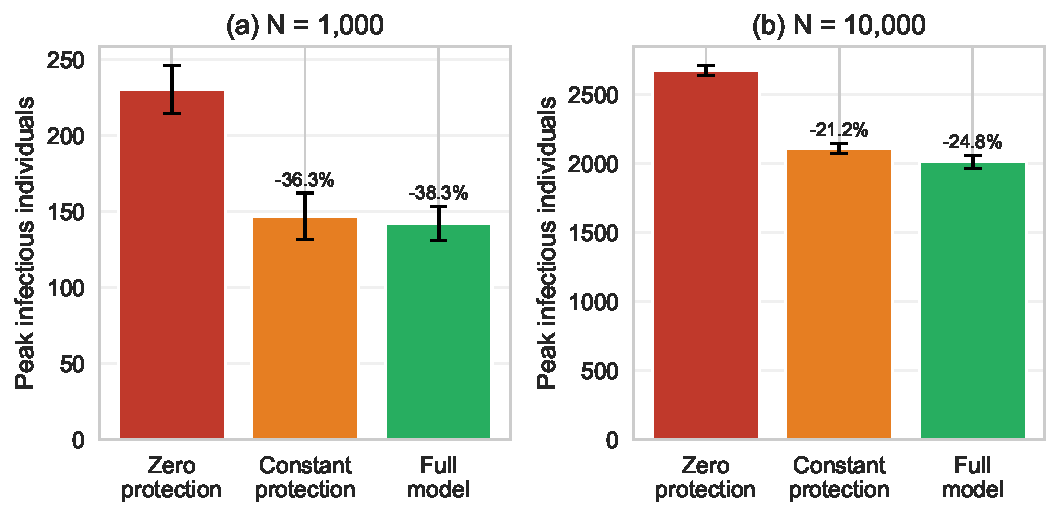
\includegraphics[width=0.95\linewidth]{figures/fig3_decomposition.pdf}
\caption{Decomposition at (a) $N{=}1{,}000$ and (b) $N{=}10{,}000$: peak infectious counts (mean $\pm$ s.d.) for zero protection, constant protection at the model's own time-averaged level, and the full dynamic model.}
\label{fig:decomp}
\end{figure}

\subsection{Whose dynamics matter? The mechanism control (RQ3)}

The small dynamic margin above could reflect a general truth about behavioural dynamics, or a property of our saliency parameterisation. The mechanism control separates the two (Table~\ref{tab:mech}). Replacing the saliency--sigmoid module with the prevalence-tracking awareness-diffusion module---same transmission skeleton, same modulation form, matched mean protection of about 0.34---more than doubles the peak reduction (49.3\% vs.\ 33.2\%) and cuts total infections by a further 6.5 percentage points, with a dynamic margin of 22.5 percentage points that is unambiguously significant ($p{=}5.5\times10^{-5}$). Skeleton equivalence was verified first: the two mechanisms' zero-protection arms are statistically indistinguishable ($221.0 \pm 12.6$ vs.\ $218.7 \pm 18.5$).

\begin{table}[htb]
\centering
\small
\begin{tabular}{llccc}
\hline
\textbf{Mechanism} & \textbf{Arm} & \textbf{Peak} & \textbf{Peak reduction} & \textbf{Dynamic margin} \\
\hline
Awareness diffusion & Zero protection & $221.0 \pm 12.6$ & --- & --- \\
 & Constant ($A \equiv \bar{A}{=}0.685$) & $144.5 \pm 13.5$ & $34.6\%$ & --- \\
 & Dynamic ($m^{*}{=}0.497$) & $112.0 \pm 14.2$ & \textbf{49.3\%} & \textbf{+22.5 pp} ($p{=}5.5{\times}10^{-5}$) \\
\addlinespace
Saliency--sigmoid (ours) & Zero protection & $218.7 \pm 18.5$ & --- & --- \\
 & Constant ($P^{*}{=}0.336$) & $148.8 \pm 13.8$ & $32.0\%$ & --- \\
 & Dynamic & $146.2 \pm 11.8$ & $33.2\%$ & +1.7 pp ($p{=}0.656$) \\
\hline
\end{tabular}
\caption{Mechanism control at matched mean protection ($N{=}1{,}000$, 10 replicates per arm, mean $\pm$ s.d.).}
\label{tab:mech}
\end{table}

The difference is the time shape of protection. The awareness module's $A(t)$ is prevalence-driven: protection rises from zero exactly as the epidemic gathers force and reaches $\bar{A}\approx0.68$ at peak, concentrating suppression where transmission is strongest. Our saliency channel, locked on the saturated shoulder of its sigmoid, produces near-flat protection throughout. The negative result and the positive control together constitute a diagnosis: the limitation of the present framework is the response-function shape, not behavioural dynamics as such.

Two robustness checks close the remaining inferential gaps. First, the awareness-control conclusion is not an artefact of one parameterisation: re-running the matched comparison over a $3\times3$ grid of the awareness parameters ($p_A \in \{0.15, 0.25, 0.35\}$, $d_A \in \{0.05, 0.1, 0.2\}$, $q$ fixed at 0.8, $m^{*}$ recalibrated per cell), the dynamic margin is positive in 8 of 9 configurations and significant in 7, ranging from +18.7 to +48.2 percentage points (Table~\ref{tab:awaresens}). The single exception ($p_A{=}0.35$, $d_A{=}0.05$) is the high-contact, slow-forgetting corner in which awareness persists near saturation, so constant protection at the matched level performs equivalently to the dynamic arm. Second, the saliency channel's small margin is not an artefact of the default midpoint: sweeping the sigmoid midpoint $\mu \in [0.3, 0.7]$ (step 0.1) and slope $\kappa \in \{1.5, 3.0\}$ (10 replicates per cell, matched-constant control per cell; the zero-protection arm is shared across cells, since with behaviour disabled the runs do not depend on the shape parameters), the dynamic margin stays between 1.3 and 5.9 percentage points and never reaches significance at any shape, although the mean protection $P^{*}$ varies from 0.126 to 0.405 across the grid (Table~\ref{tab:shape}). The amplitude difference is visible directly in the protection paths: over the whole epidemic, the saliency channel's population protection moves within a band of width only 0.05 (0.321 to 0.370), whereas the awareness module's sweeps 0.49 (0.004 to 0.497). The saliency-to-protection mapping compresses the dynamics into a narrow band at every tested shape; the awareness module's prevalence-tracking dynamics have both the amplitude and the timing that the saliency channel lacks.

\begin{table}[htb]
\centering
\small
\begin{tabular}{lccc}
\hline
$p_A \backslash d_A$ & 0.05 & 0.10 & 0.20 \\
\hline
0.15 & +18.7 pp$^{*}$ & +35.7 pp$^{*}$ & +40.0 pp$^{*}$ \\
0.25 & +3.9 pp (n.s.) & +28.2 pp$^{*}$ & +48.2 pp$^{*}$ \\
0.35 & $-0.8$ pp (n.s.) & +23.6 pp$^{*}$ & +41.5 pp$^{*}$ \\
\hline
\end{tabular}
\caption{Dynamic margin of the awareness module across its parameter grid ($m^{*}$ recalibrated per cell; $^{*}$ significant at $p<0.05$, Welch $t$, 5 replicates per arm).}
\label{tab:awaresens}
\end{table}

\begin{table}[htb]
\centering
\small
\begin{tabular}{lcccc}
\hline
 & $\mu{=}0.3$ & $\mu{=}0.4$ & $\mu{=}0.5$ & $\mu{=}0.6$ \\
\hline
$\kappa{=}1.5$: $P^{*}$ / margin (pp) & 0.405 / +4.2 & 0.370 / +4.1 & 0.336 / +3.4 & 0.304 / +1.3 \\
$\kappa{=}3.0$: $P^{*}$ / margin (pp) & 0.319 / +4.6 & 0.258 / +5.9 & 0.206 / +3.8 & 0.161 / +1.6 \\
\hline
\end{tabular}
\caption{Response-shape sweep: mean protection $P^{*}$ and the saliency channel's dynamic margin (all non-significant, $p \ge 0.18$); $\mu{=}0.7$ cells are omitted here and reported in the archived outputs ($P^{*}{=}0.273/0.126$; margins $+2.6$/$+2.3$ pp).}
\label{tab:shape}
\end{table}

\subsection{Media amplification and the 20\% target (RQ4)}

Across $\alpha \in \{0.5,\dots,5\}$ (10 replicates per group), peak reductions relative to $\alpha{=}0.5$ stay modest (Table~\ref{tab:alpha}), while maximum protection rises monotonically from 0.357 to 0.458. A threshold search over $\alpha \in [0.5, 10]$ (step 0.5, 5 replicates per point) finds the pre-specified target of a 20\% peak reduction first met at $\alpha{=}5.0$ (21.9\%), reaching at most 30.4\% at $\alpha{=}10$. The target was fixed before the sensitivity study in the project's research protocol; operationally, a 20\% peak reduction corresponds to roughly a fifth of peak-day admission and testing demand---the scale at which bed-capacity decisions become material. Since $\alpha{=}5$ denotes ten-fold amplification relative to the reference, the practical reading is that intensifying media amplification alone is a low-leverage instrument in this parameterisation; protection rising 28\% translates into at most a 20\% peak reduction.

\begin{table}[htb]
\centering
\small
\begin{tabular}{lccccc}
\hline
$\alpha$ & \textbf{Peak} & \textbf{Peak reduction} & \textbf{Total} & \textbf{Peak day} & \textbf{Max protection} \\
\hline
0.5 & $150.0 \pm 17.3$ & 0.0\% (ref.) & $885.4 \pm 18.6$ & 65.7 & 0.357 \\
1.0 & $135.6 \pm 16.4$ & 9.60\% & $875.3 \pm 16.3$ & 66.2 & 0.367 \\
1.5 & $142.7 \pm 10.8$ & 4.87\% & $872.4 \pm 12.6$ & 65.0 & 0.383 \\
2.0 & $138.1 \pm 19.5$ & 7.93\% & $873.7 \pm 23.0$ & 66.6 & 0.394 \\
3.0 & $134.2 \pm 10.7$ & 10.53\% & $865.0 \pm 17.5$ & 66.7 & 0.419 \\
5.0 & $120.0 \pm 13.3$ & \textbf{20.00\%} & $846.0 \pm 22.4$ & 66.2 & 0.458 \\
\hline
\end{tabular}
\caption{Media-amplification sensitivity (10 replicates per group, mean $\pm$ s.d.; reference $\alpha{=}0.5$).}
\label{tab:alpha}
\end{table}

A complementary sweep of the behavioural parameters (10 replicates per cell against a zero-protection reference on the same seed set; Table~\ref{tab:kappa}) shows that the switch effect is robust to the response sensitivity and inertia at flattest responses ($\kappa{=}0.5$: 46.5--47.8\%; $\kappa{=}1.0$: 40.0--40.9\% across $\eta \in \{0, 0.15, 0.3, 0.5\}$), decays for steeper responses ($\kappa{=}1.5$: 31.5--35.2\%; $\kappa{=}2$: 25--29\%; $\kappa{=}3$: 19--21\%), and is nearly insensitive to inertia (at most 3.7 percentage points within any $\kappa$ row). The mechanism mirrors the decomposition: a steeper sigmoid lowers the low-risk baseline protection, which---not the information dynamics---is what carries the effect.

\begin{table}[htb]
\centering
\small
\begin{tabular}{lcccc}
\hline
$\kappa \backslash \eta$ & 0.00 & 0.15 & 0.30 & 0.50 \\
\hline
0.5 & 46.5 & 47.8 & 47.8 & 47.8 \\
1.0 & 40.7 & 40.9 & 40.5 & 40.0 \\
1.5 & 35.2 & 34.5 & 34.6 & 31.5 \\
2.0 & 25.8 & 25.4 & 25.7 & 28.7 \\
3.0 & 21.0 & 21.2 & 20.0 & 18.9 \\
\hline
\end{tabular}
\caption{Peak reduction (\%) against a zero-protection reference, across response sensitivity $\kappa$ and behavioural inertia $\eta$ (10 replicates per cell).}
\label{tab:kappa}
\end{table}

\subsection{Calibration and seasonal transfer (RQ5)}

Grid search on the deterministic surrogate fits the Brazilian 2019 weekly series closely: $\beta{=}0.25$, $\sigma{=}0.1$, $\gamma{=}0.1$, $\alpha{=}1.0$, $I_0{=}5{\times}10^{5}$, with reporting fraction $\rho{=}0.0114$, RMSE 10{,}078 weekly cases, $R^{2}{=}0.941$, and human-channel $R_0{=}2.50$ (Figure~\ref{fig:calib}). One interpretive caveat must accompany these numbers: the fitted parameters calibrate the model \emph{as specified}---a system whose transmission is dominated by the direct human-to-human term (Section 4.6)---and should therefore be read as parameters of this model structure, not as dengue-specific biology. The fitted parameters reproduce the agent model faithfully (weekly-incidence correlation $r{=}0.967$; 96\% of weeks have an ABM mean incidence within the surrogate value $\pm$ 2 across-run standard deviations, with an additional 5\%-of-surrogate tolerance), so the surrogate is a valid fast stand-in. Three caveats are reported rather than smoothed over. First, $\sigma$ sits on the grid boundary (a 10-day incubation period, above the 4--7 days typical of dengue): without seasonal forcing, the model compensates with slower dynamics, and the fitted $\sigma$ must not be read biologically. Second, $\rho$ is a fitted effective reporting rate, not an independent measurement. Third, out-of-season transfer is bounded (Table~\ref{tab:seasons}): freezing the dynamics and re-solving only $\rho$ yields $R^{2}=0.944$ (2022), $0.788$ (2023), $0.563$ (2021), and $0.117$ (2016), but fails in the small epidemic year 2017 ($-0.097$) and the atypical year 2018 ($-0.530$); allowing per-season $I_0$ rescues 2016 (0.868) but not 2017--2018. The calibration therefore transfers to seasons shaped like the training season and fails where the shape differs---the honest boundary of a seasonally unforced model.

\begin{table}[htb]
\centering
\small
\begin{tabular}{lccc}
\hline
\textbf{Season} & \textbf{Reported cases} & \textbf{Strict $R^2$ (frozen $I_0$)} & \textbf{Loose $R^2$ (per-season $I_0$)} \\
\hline
2016 & 2.22M & 0.117 & 0.868 \\
2017 & 0.51M & $-0.097$ & 0.248 \\
2018 & 0.47M & $-0.530$ & $-0.437$ \\
\textbf{2019} & \textbf{2.25M} & \textbf{0.941} (in-sample) & 0.941 \\
2021 & 0.98M & 0.563 & 0.563 \\
2022 & 2.36M & 0.944 & 0.944 \\
2023 & 3.15M & 0.788 & 0.788 \\
\hline
\end{tabular}
\caption{Frozen-parameter transfer across Brazilian seasons (2020 missing from the extract).}
\label{tab:seasons}
\end{table}

\begin{figure}[htb]
\centering
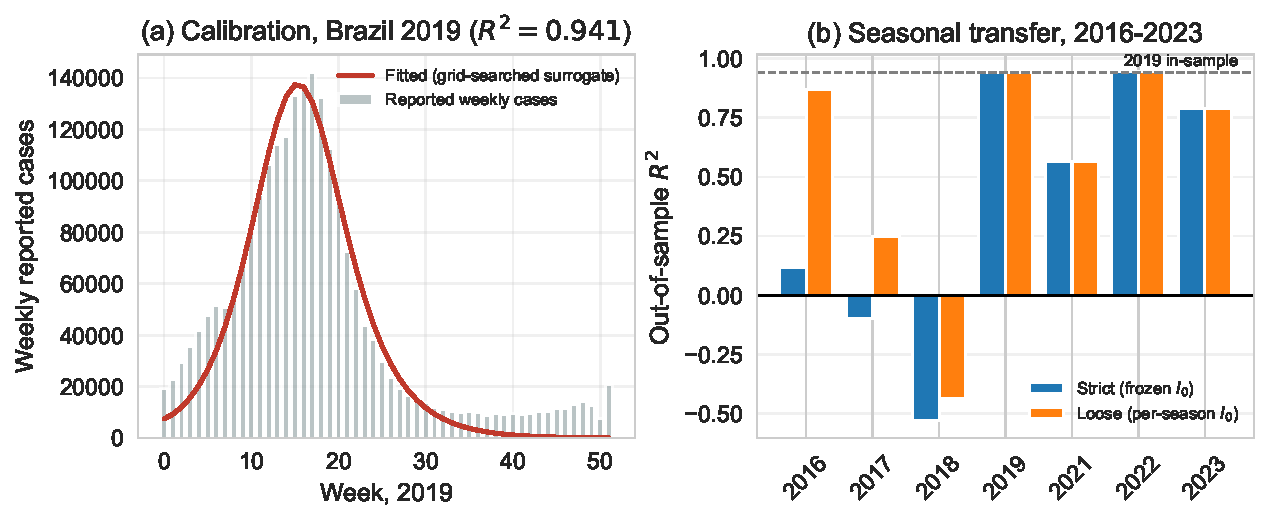
\includegraphics[width=0.98\linewidth]{figures/fig4_calibration.pdf}
\caption{(a) Grid-searched surrogate fit to Brazil 2019 weekly reported cases. (b) Frozen-parameter transfer across seasons (strict: $I_0$ frozen; loose: per-season $I_0$), with the in-sample $R^2$ dashed.}
\label{fig:calib}
\end{figure}

\subsection{Component ablation (RQ6)}

Six conditions under paired seeds (beds tightened to 50 and ICU to 10 so the constraint binds; $\alpha{=}1.5$) attribute system behaviour to components (Table~\ref{tab:ablation}). Removing the behavioural feedback raises the peak by 47.4\% and deferred admissions by 113\%---the load-bearing component. Removing the information-saliency channel alone changes the peak by $-3.2\%$, i.e.\ not at all within paired noise, even though peak protection drops 7.8\%: consistent with the decomposition, a 0.03 improvement in mean protection carries no epidemiological leverage here. Removing the hospital constraint leaves every transmission metric exactly unchanged---admission does not isolate infectious agents, so beds do not touch the epidemic---and affects only deferred admissions ($203 \to 0$). An earlier version of this study reported an 18\% peak effect of removing the constraint; that was an artefact of attributing single-run random-stream divergence to a component, which the paired-seed design eliminates. Removing the mosquito channel lowers the peak by 5.4\% at this $\alpha$. Removing the human-to-human term instead collapses the epidemic entirely---the peak equals the ten initially infected agents in every replicate (a 93.3\% reduction), with no sustained mosquito-borne chain---so in the present parameterisation the direct-transmission simplification carries essentially all transmission. This is an honest quantification of how far the model currently sits from a vector-borne disease's true transmission structure, and it flags mosquito-channel calibration as the most consequential model-development task. Deferred admissions is the DES layer's useful output: 203, 0, and 432 across scenarios---resource pressure responds to intervention scenarios even though transmission does not.

\begin{table}[htb]
\centering
\small
\begin{tabular}{lcccc}
\hline
\textbf{Condition} & \textbf{Peak} & \textbf{Total infected} & \textbf{Peak protection} & \textbf{Deferred admissions} \\
\hline
Baseline & $149.7 \pm 14.0$ & $887.3 \pm 17.9$ & $0.371$ & $202.7 \pm 61.6$ \\
No saliency & $144.9 \pm 11.8$ & $892.8 \pm 15.2$ & $0.342$ & $196.5 \pm 42.9$ \\
No behavioural feedback & $220.6 \pm 17.9$ & $967.4 \pm 7.3$ & $0.000$ & $432.0 \pm 33.7$ \\
No hospital constraint & $149.7 \pm 14.0$ & $887.3 \pm 17.9$ & $0.371$ & $0.0 \pm 0.0$ \\
No mosquito channel & $141.6 \pm 18.6$ & $839.4 \pm 32.4$ & $0.369$ & $147.5 \pm 61.5$ \\
No human-to-human term & $10.0 \pm 0.0$ & $14.2 \pm 3.0$ & $0.324$ & $0.0 \pm 0.0$ \\
\hline
\end{tabular}
\caption{Component ablation (6 conditions $\times$ 10 paired-seed replicates; beds 50, ICU 10; mean $\pm$ s.d.).}
\label{tab:ablation}
\end{table}

\section{Discussion}

\subsection{The level carries the effect; the design reveals it}

Across a switch comparison, a constant-protection decomposition, a single-channel ablation, and a population-scale replication, one conclusion is stable: in this framework, the epidemiological effect of endogenous protective behaviour is carried almost entirely by the protection \emph{level}, not by its information-driven dynamics---95\% at $N{=}1{,}000$, 85\% at $N{=}10{,}000$. The scale replication matters for how the headline should be read: absolute peak reductions shrink from 35.9\% to 24.8\% as the small-population stochastic attenuation disappears, and the dynamic margin, invisible at the smaller scale, becomes significant but minor. Behaviour-coupled epidemic models that report only with-versus-without comparisons should be read with this in mind; we initially mis-attributed our own effect in exactly that way, and the decomposition design is the correction.

\subsection{Diagnosing the mechanism, not just the number}

The mechanism control turns the negative result into a constructive diagnosis. At matched mean protection, a prevalence-tracking awareness module extracts a large, significant dynamic margin where the saliency--sigmoid module extracts none, and the response-shape sweep shows the saliency margin stays negligible across every tested midpoint and slope. This is the simulation-side counterpart of Fenichel et al.'s theoretical argument that adaptive behaviour changes epidemic predictions \cite{fenichel2011adaptive}: whether behaviour \emph{dynamics} matter depends on how the behaviour module maps information to protection. Prevalence-coupled protection---rising as the epidemic gathers force---times the suppression to where transmission is strongest; a mapping whose dynamic range is narrow cannot, regardless of where its curve sits. The actionable implication for our framework is specific: give the saliency-to-protection mapping a wider dynamic range by coupling the protection target to prevalence (the awareness module's route), or recalibrate the response function against empirical risk--protection data, before drawing any conclusion about information-driven dynamics. More generally, the decomposition plus mechanism-control pair is a portable diagnostic: it tells a modeller \emph{which part} of a behavioural mechanism deserves design attention.

\subsection{Calibration is trustworthy only within its transfer boundary}

The surrogate-based calibration achieved $R^{2}=0.941$ on Brazilian 2019 data with a plausible fitted reporting rate, and the surrogate itself reproduces the agent model closely. The out-of-season tests then did their job: large epidemic seasons transfer ($R^{2}=0.79$--$0.94$), small and atypical years do not. A seasonally unforced model cannot represent inter-annual shape variation, and the fitted $\sigma$ sitting on its grid boundary is the visible signature of that compensation. We therefore read the calibration as ``single-season fit plus shape-matched transfer'', not as predictive validity, and we treat the multi-season test as a template: a calibration claim without a frozen-parameter transfer test is unbounded.

\subsection{The DES boundary is a design fact, not a defect}

The ablation quantifies an architectural property: hospital capacity does not influence transmission because admission does not isolate infectious agents. The DES layer's value in this framework is resource-pressure analytics---deferred admissions swing from 0 to 432 across scenarios---which is precisely what bed-planning decisions need. Coupling admission to transmissibility (isolation reducing onward transmission) would give the resource layer epidemiological leverage and is the natural next extension; until then, transmission forecasting and capacity planning should use different layers of the same model, and the ablation is what makes that split defensible.

\subsection{Limitations}

\subsection{Limitations and threats to validity}

Five limitations bound the claims. First, the human-to-human transmission term is a simplification standing in for unmodelled pathways in a primarily vector-borne disease, and the ablation shows it currently carries almost all transmission (Section 4.6): a mosquito-only (Ross--Macdonald-style) parameterisation that can sustain transmission is the principled reformulation, and recalibrating the mosquito channel is the most consequential development task. Second, mixing is homogeneous: no spatial structure, contact networks, or individual heterogeneity in behaviour. Third, the behaviour module's sigmoid midpoint and slope are design choices, not calibrated quantities---and Section 4.3 shows the saliency mapping's narrow dynamic range persists across the tested shapes. Fourth, the saliency signal is a global scalar with uncalibrated media parameters; its decay is indexed to calendar time, which is valid only within a single wave. Fifth, individual-level validation stops at $N{=}10^{4}$, far below city or national scale, and the calibration covers one country and seven seasons. The awareness-diffusion control is a representative implementation of a mechanism class, not a reproduction of any specific published model; its conclusion is robust across the tested parameter grid, but its own parameters were not optimised.

In threat-to-validity terms: \emph{construct} validity is limited by the parsimonious saliency proxy (no media data) and the global-scalars signal; \emph{internal} validity is protected by the seeded paired design and the consistency checker, with the residual threat that the awareness control's parameters, though swept, were not fitted to any empirical awareness process; \emph{external} validity is bounded by the single country, the seven seasons, the homogeneous mixing, and the $10^{3}$--$10^{4}$ population scale, with the scale replication indicating which conclusions are scale-sensitive (peak magnitudes) and which are not (the level-versus-dynamics ordering).

\subsection{Future work}

Four extensions follow directly from the findings. Coupling admission to transmissibility so that the DES layer carries epidemiological leverage. Redesigning the response function with prevalence-coupled protection targets, per the mechanism diagnosis. Adding seasonal mosquito dynamics and multi-season calibration windows, which the transfer tests show is where the calibration fails. And calibrating the saliency parameters $\alpha$ and $\lambda$ against real media-attention data, completing the measurement story that the present formalisation deliberately leaves open.

\section{Conclusion}

We presented a four-layer hybrid simulation framework for dengue---agents, transmission dynamics, hospital resources, and explicit mosquito dynamics---and an effect-decomposition evaluation design that separates what a behaviour-coupled model \emph{is} from what its dynamics \emph{do}. Under a seeded, mechanically verified regeneration protocol, the framework's information-driven behavioural feedback flattens the simulated epidemic, but 85--95\% of that effect is reproduced by a constant protection level; the saliency-driven dynamics add little, a mechanism control shows this is a fixable property of the response function rather than a law of behavioural dynamics, and calibration transfers to seasons shaped like the training season but not beyond. For builders of behaviour-coupled epidemic models, the decomposition design---constant-protection control, mechanism control, paired-seed ablation, frozen-parameter transfer tests---is inexpensive and, we argue, should be part of the standard evaluation toolkit; for decision-makers, the practical message is that raising and sustaining population protection is the high-leverage intervention, while amplifying media intensity alone is not.

\section*{Declaration of generative AI use}

Generative AI tools were used in this work: in developing the simulation code, executing and documenting the seeded experiment protocol, and in drafting and translating the manuscript. All quantitative results were produced by the deterministic, seeded experiment protocol described in the paper and verified by an automated consistency check; the authors reviewed and take full responsibility for the content of the published article.

\section*{Declaration of interest statement}

The authors report there are no competing interests to declare.

\section*{Funding}

This work received no external funding.

\section*{Data availability statement}

The dengue surveillance data are publicly available from the OpenDengue project (national-level extract v1.3, \url{https://opendengue.org/data.html}) \cite{opendengue2024}. An anonymized repository containing the full simulation code, experiment scripts, run manifests, consistency checker, and the archived output files that reproduce every figure and table in this paper is publicly available at \url{https://github.com/7Dt3V5TmzAtfur/HybridSimulation-InfoSaliency} for the duration of double-anonymous review; upon acceptance the repository will be archived with a persistent identifier.

\appendix

\section{Regeneration protocol and consistency checking}

Every experiment runs under a common protocol: independent seeds per replicate ($s = 1000\,b + i$, with per-experiment base seeds $b$), canonical result-file names, and an appended run manifest recording the code commit, seeds, protocol parameters, and dependency versions for each rerun. A consistency script re-derives the manuscript's key quantitative claims directly from the archived CSV outputs, checks manifest coverage and code-version anchoring, and is wired as a local pre-commit hook so that a commit whose numbers do not match the archived results is rejected. The results underlying this manuscript were generated in a single pass on the anchored code revision and verified byte-identical under a full seeded re-run. The two-stage submission artefacts (code commit, then re-run-anchored results commit) keep the paper, the results, and the code version in one verifiable chain.

\section{Proofs}\label{app:proofs}

\subsection*{Proof of Lemma~\ref{lem:envelope}}
By definition, $\bar{R}(t) = w_{\mathrm{info}} S(t) + w_{\mathrm{soc}}\, I(t)/N + w_{\mathrm{pers}}\,(E(t)+I(t))/N$ averaged over agents, with all weights nonnegative. Since $S(t) = \min(1, (I(t)/N)\,\alpha\, e^{-\lambda t/100}) \le (I(t)/N)\,\alpha$ and $(E+I)/N \le 1$, each term is nonnegative and bounded by its share of $\bar{R}_{\max}$; summing gives the envelope. $\square$

\subsection*{Proof of Proposition~\ref{prop:threshold}}
Linearise the expected dynamics at the disease-free state $(s,e,i,r)=(1,0,0,0)$, $\bar{P}$ constant. With $\bar{P}$ constant, both transmission channels scale by the factor $(1-\varepsilon\bar{P})$: the direct channel through $\beta_{\mathrm{eff}}$, the mosquito channel through the modulation of the mosquito-induced hazard. The daily transition matrix of the linearised state $(e, i, m_e, m_i)$ (fractions of $N$ and $M$ respectively) is
\[
M = \begin{pmatrix}
1-\sigma & (1-\varepsilon\bar{P})\beta & 0 & (1-\varepsilon\bar{P})\,b\,p_{mh}\\
\sigma & 1-\gamma & 0 & 0\\
0 & (1-\varepsilon\bar{P})\,b\,p_{hm}\tfrac{N}{M} & 1-\tfrac{1}{\mathrm{EIP}} & 0\\
0 & 0 & \tfrac{1}{\mathrm{EIP}} & 1-\tfrac{1}{L}
\end{pmatrix}.
\]
Split $M = F + T$ into the new-infection part $F$ (entries $F_{e i} = (1-\varepsilon\bar{P})\beta$, $F_{e m_i} = (1-\varepsilon\bar{P}) b p_{mh}$, $F_{m_e i} = (1-\varepsilon\bar{P}) b p_{hm} \tfrac{N}{M}$) and the transition part $T$. The next-generation matrix is $K = F(I-T)^{-1}$, whose nonzero block is
\[
K = \begin{pmatrix}
(1-\varepsilon\bar{P})\tfrac{\beta}{\gamma} & (1-\varepsilon\bar{P})\, b\,p_{mh}\,L\\
(1-\varepsilon\bar{P})\,\tfrac{b\,p_{hm}}{\gamma}\tfrac{N}{M} & 0
\end{pmatrix},
\]
using $(I-T)^{-1}_{e i} = 1/\gamma$, $(I-T)^{-1}_{m_i m_i} = L$ (an infectious mosquito causes $b\,p_{mh}$ human exposures per day over its $L$-day life) and $(I-T)^{-1}_{m_e i} = 1/\gamma$. The spectral radius of the $2\times2$ block is
\[
R_{\mathrm{eff}}(\bar{P}) = (1-\varepsilon\bar{P})\,\frac{K_h + \sqrt{K_h^2 + 4K_{hv}K_{vh}}}{2},
\]
with $K_h = \beta/\gamma$, $K_{hv} = (b\,p_{hm}/\gamma)(N/M)$, $K_{vh} = b\,p_{mh}\,L$. Setting $\bar{P}=0$ gives Proposition~\ref{prop:threshold}; the invasion condition $R_{\mathrm{eff}} > 1$ rearranges to Corollary~\ref{cor:block}. The dominant eigenvalue of $M$ at $\bar{P}=0$ is the theoretical early growth factor per day, compared with simulation in Table~\ref{tab:theory}. $\square$

\subsection*{Proof of Proposition~\ref{prop:band}}
Individual risk $R_i(t)$ is a convex combination of nonnegative bounded terms, so $0 \le R_i(t) \le \bar{R}_{\max}$ (Lemma~\ref{lem:envelope}). Since $\sigma$ is strictly increasing, $\sigma(-\kappa\mu) \le P_i(t) \le \sigma(\kappa(\bar{R}_{\max}-\mu))$, and the population mean inherits the same bounds. For the width: writing $\Delta = \kappa \bar{R}_{\max}$, the function $g(x) = \sigma(x+\Delta) - \sigma(x)$ satisfies $g'(x) = 0$ exactly at $x = -\Delta/2$, where $g = \sigma(\Delta/2) - \sigma(-\Delta/2) = \tanh(\Delta/4)$; $g$ increases for $x < -\Delta/2$ and decreases after, so the bound is the supremum. The logit of $P_i$ is $\kappa(R_i - \mu)$, whose range $\kappa \bar{R}_{\max}$ does not involve $\mu$; hence midpoint invariance. $\square$

\bibliographystyle{tfp}
\bibliography{refs}

\end{document}
